\documentclass[12pt]{article}
\usepackage{algorithmicx}
\usepackage[ruled]{algorithm}
\usepackage{algpseudocode}
\usepackage{algpascal}
\usepackage{algc}
\usepackage{url,enumerate, amssymb, anysize, booktabs, amsfonts}
\usepackage[colorlinks = true,
linkcolor = blue,
urlcolor  = blue,
citecolor = green,
anchorcolor = blue]{hyperref}
\usepackage{setspace,listings}
\usepackage[dvipdfmx]{graphicx}
\usepackage{amsmath}
\usepackage{psfrag}
\usepackage[font=small,labelfont=bf]{caption}
\usepackage{enumerate}
\usepackage{natbib, subcaption}
\usepackage{url} % not crucial - just used below for the URL 
\usepackage{sidecap}
\sidecaptionvpos{figure}{c}
\begin{document}
	
	\title{Testing independence between networks and nodal attributes via multiscale metrics}	
		
%%%%%%%%%%%%%%%%%%%%%%%%%%%%%%%%%	
\subsection*{Introducing network topology}

\begin{figure}[H]
	\centering
	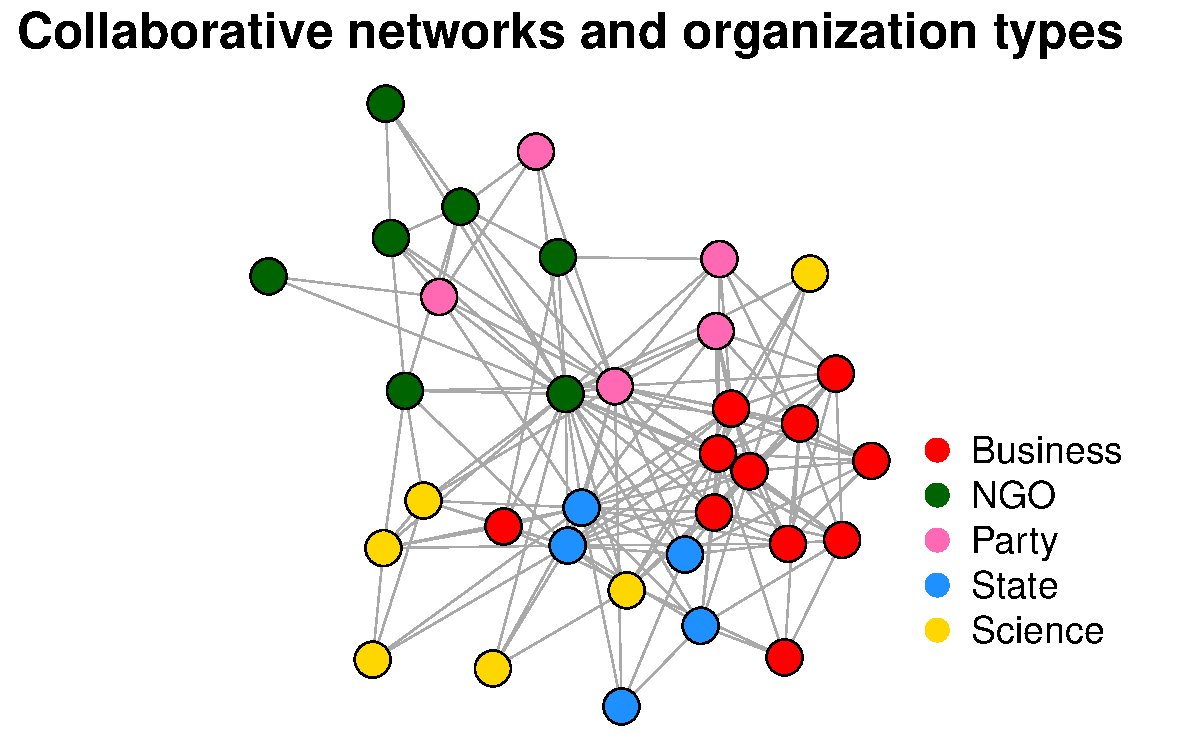
\includegraphics[width=3in]{../Figure/introplot.pdf}	
	\label{fig:intro}
	\caption{You may conjecture that organizations with the same type are more likely to collaborate each other at first glance; but there has been a lack of statistical method to \textbf{test if there exists any significant relationship between network topology and node-specific attributes and if any, which node exerts the most dependency on network.}}
\end{figure}



\subsection*{Introducing two simple Euclidean distance matrix in the context of network}

\begin{figure}[H]
	\centering
	\begin{subfigure}[b]{0.23\textwidth}
		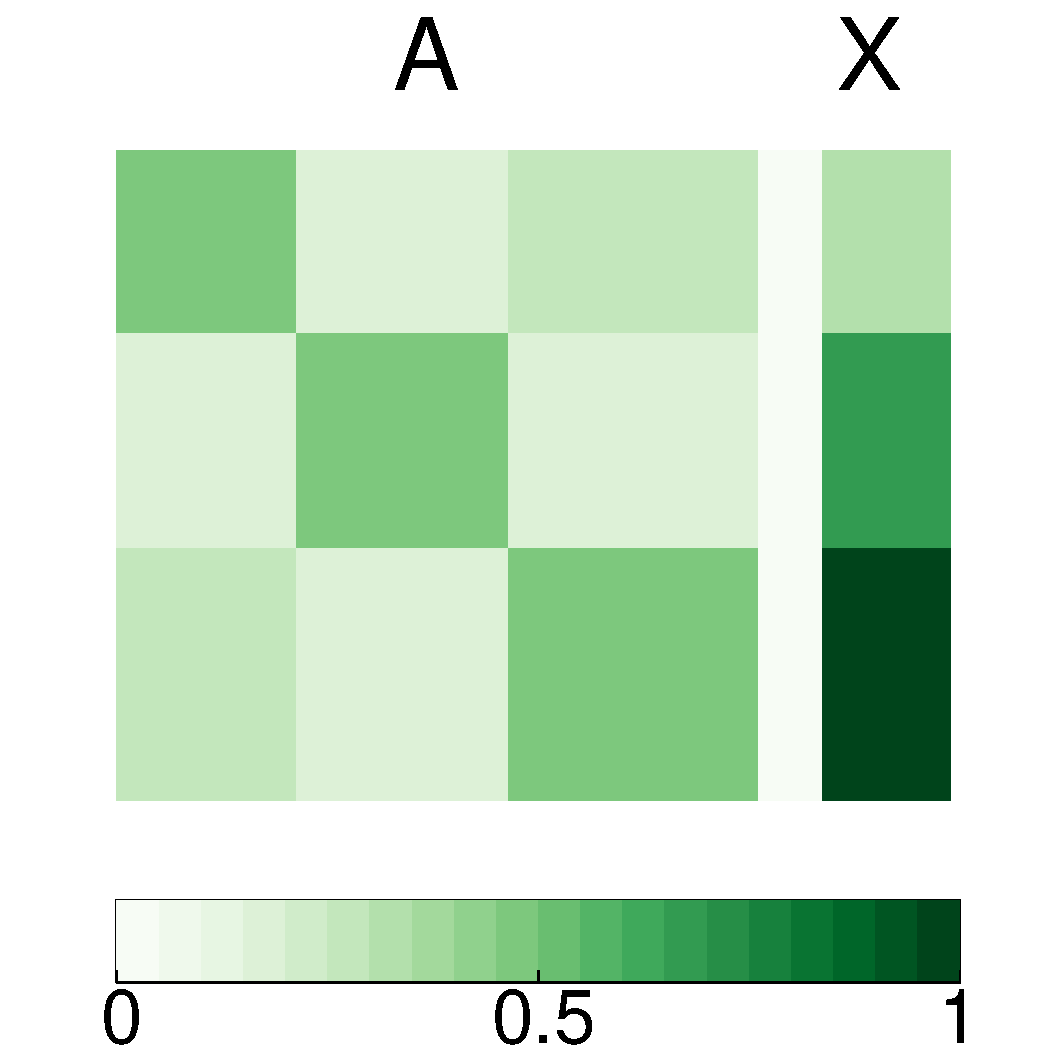
\includegraphics[width=\textwidth]{../Figure/Pmat.pdf}
		\caption{}
		\label{fig:a}
	\end{subfigure}
	~ %add desired spacing between images, e. g. ~, \quad, \qquad, \hfill etc. 
	%(or a blank line to force the subfigure onto a new line)
	\begin{subfigure}[b]{0.23\textwidth}
		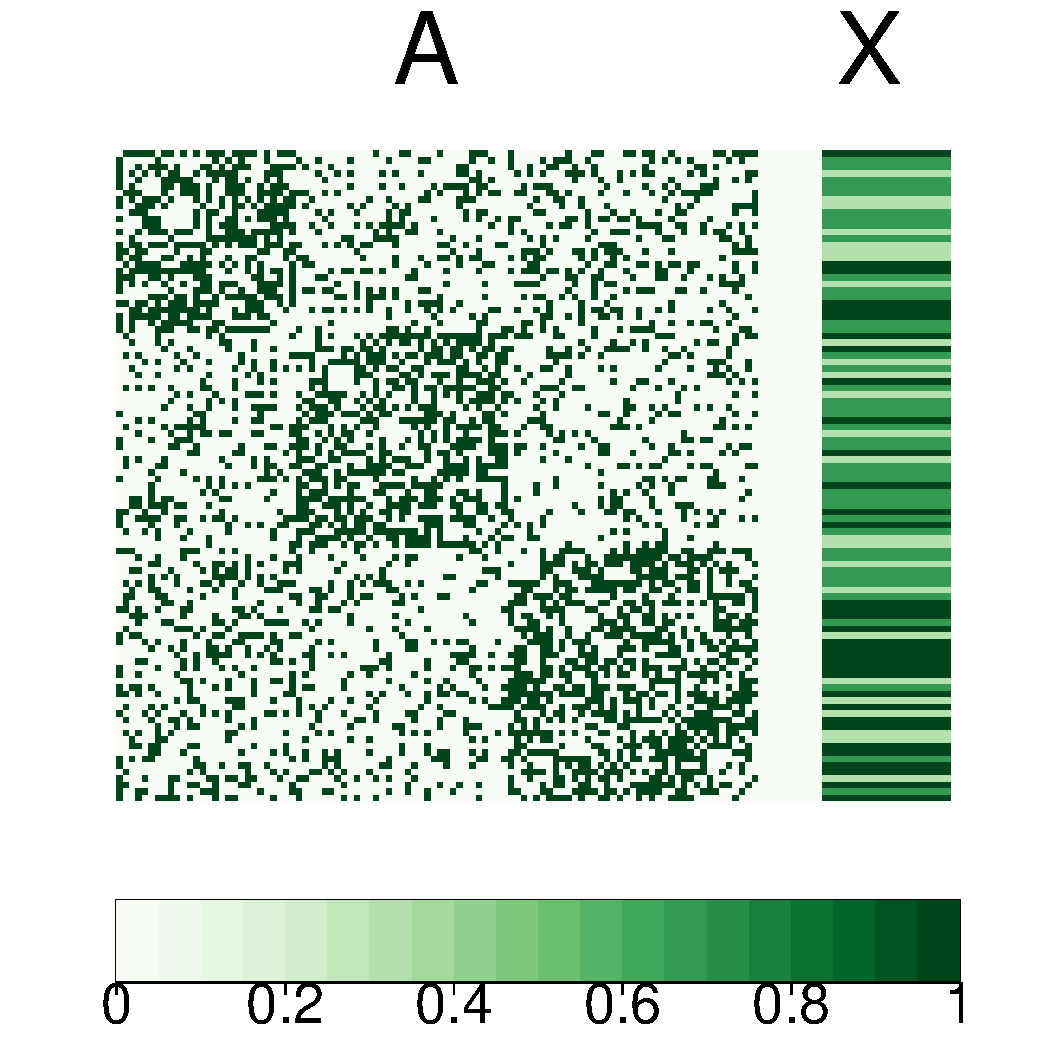
\includegraphics[width=\textwidth]{../Figure/Amat.pdf}
		\caption{}
		\label{fig:b}
	\end{subfigure}
	~ %add desired spacing between images, e. g. ~, \quad, \qquad, \hfill etc. 
	%(or a blank line to force the subfigure onto a new line)
	\begin{subfigure}[b]{0.23\textwidth}
		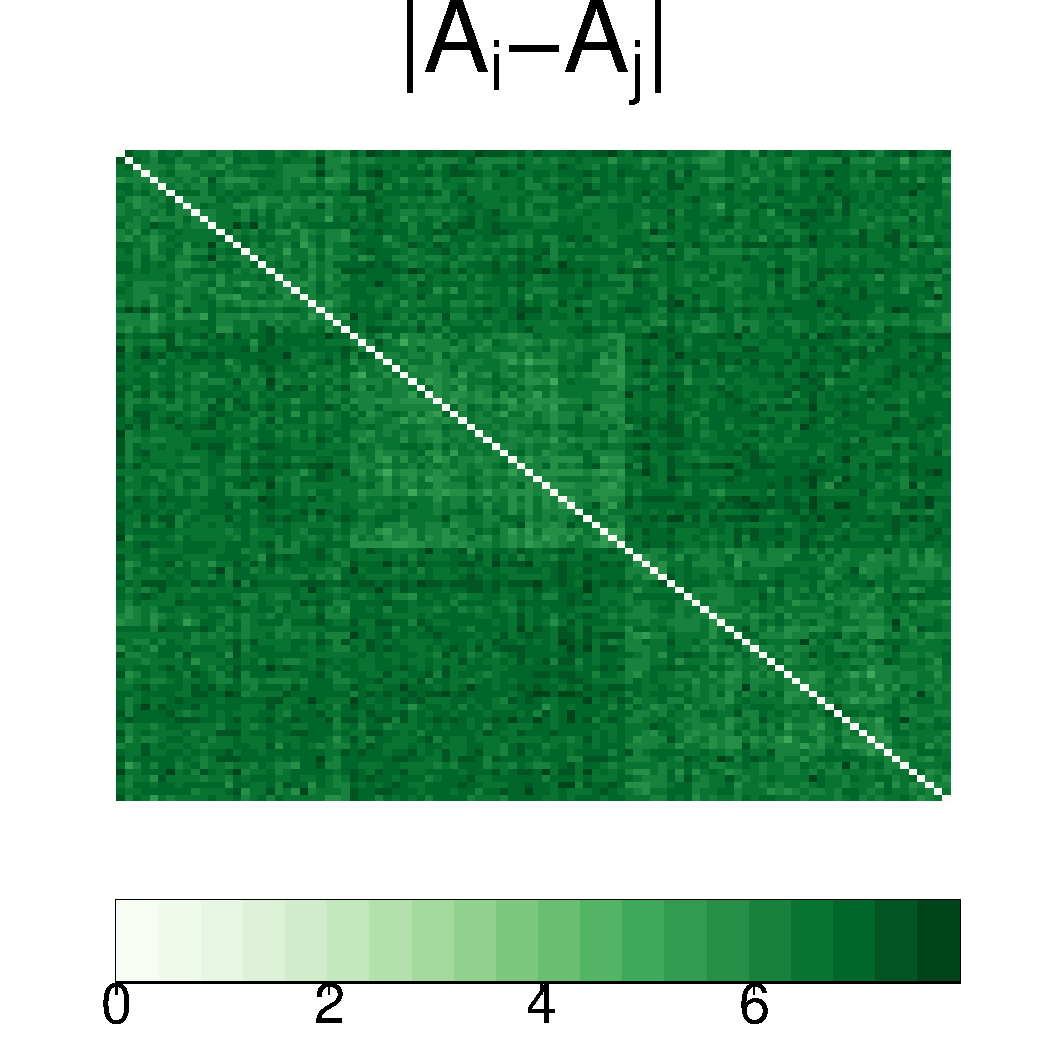
\includegraphics[width=\textwidth]{../Figure/distA.pdf}
		\caption{}
		\label{fig:c}
	\end{subfigure}
	\begin{subfigure}[b]{0.23\textwidth}
		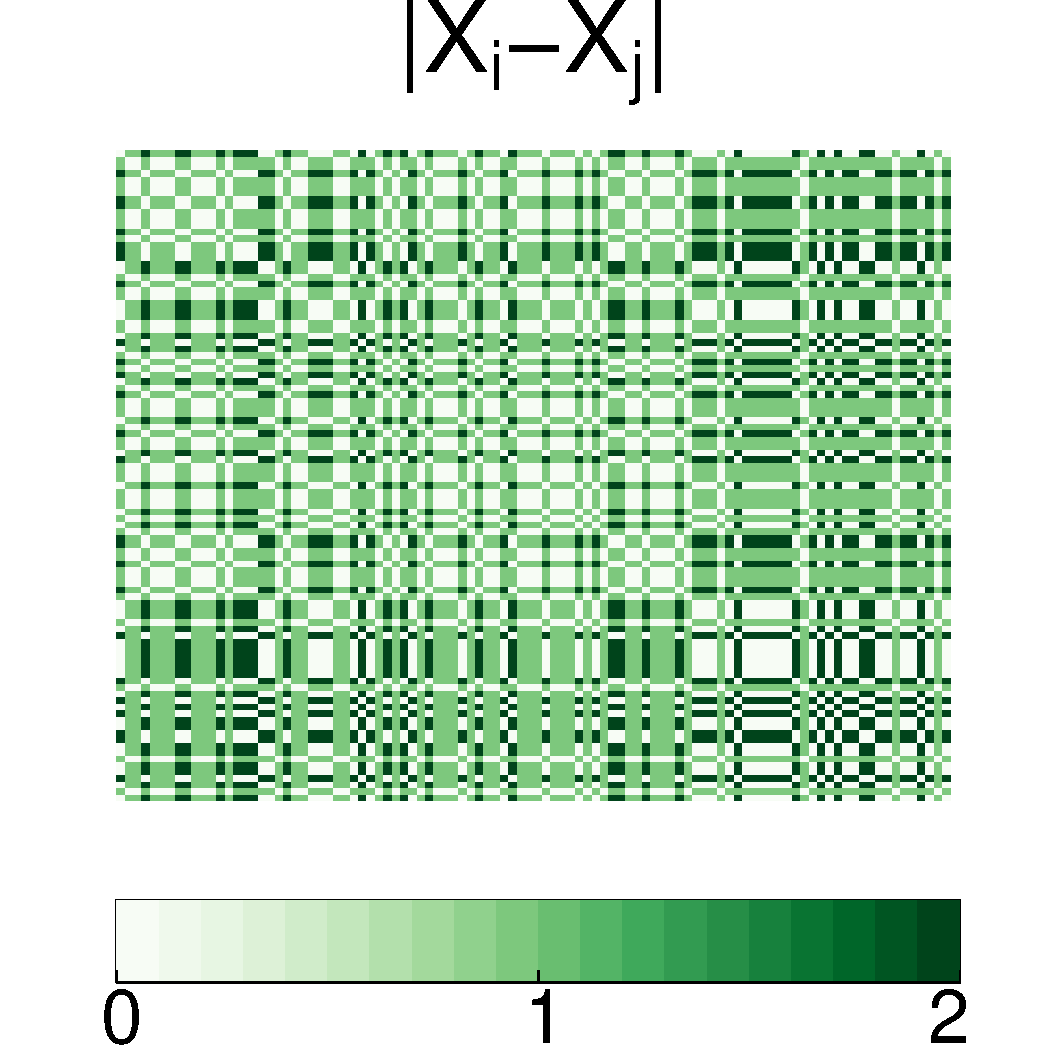
\includegraphics[width=\textwidth]{../Figure/distX.pdf}
		\caption{}
		\label{fig:d}
	\end{subfigure}
	\caption{Assume that a set of edges follow certain stochastic block model, also depending on the distribution function of nodal attributes $X$ (a), then with some amount of noise we have a realized adjacency matrix and a set of attribute outcomes (b) of which Euclidean distances ((c) and (d)) are suggested to be used in standard distance-based independence test \textbf{but neither of them manifests block structures evident in the data generating model and each column (or row) of an adjacency matrix is constructed dependently on the others.}}
	\label{fig:matrics}
\end{figure}	

\subsection*{Introduce a family of network distance matrices} 

\begin{figure}[H]
	\centering
	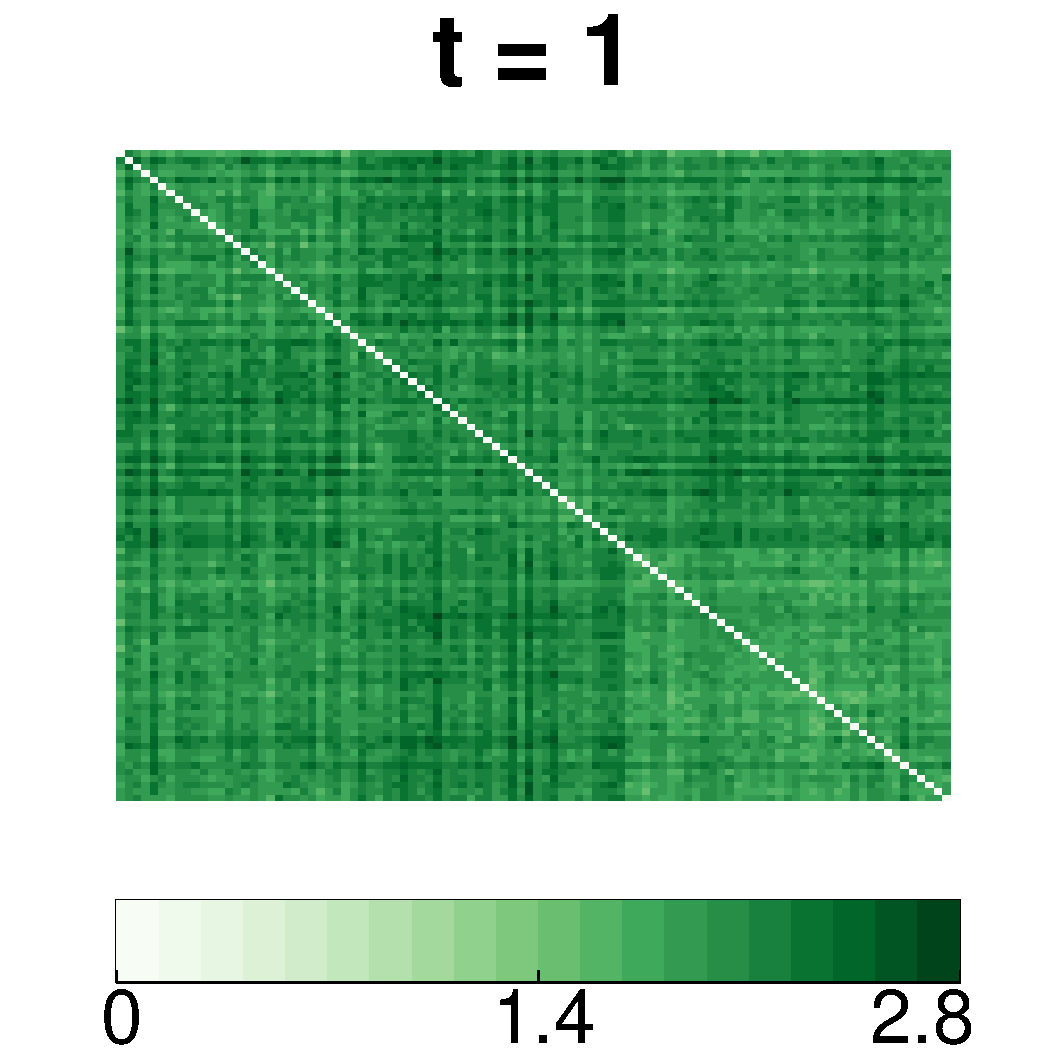
\includegraphics[width=0.3\linewidth]{../Figure/Dx1.pdf}
	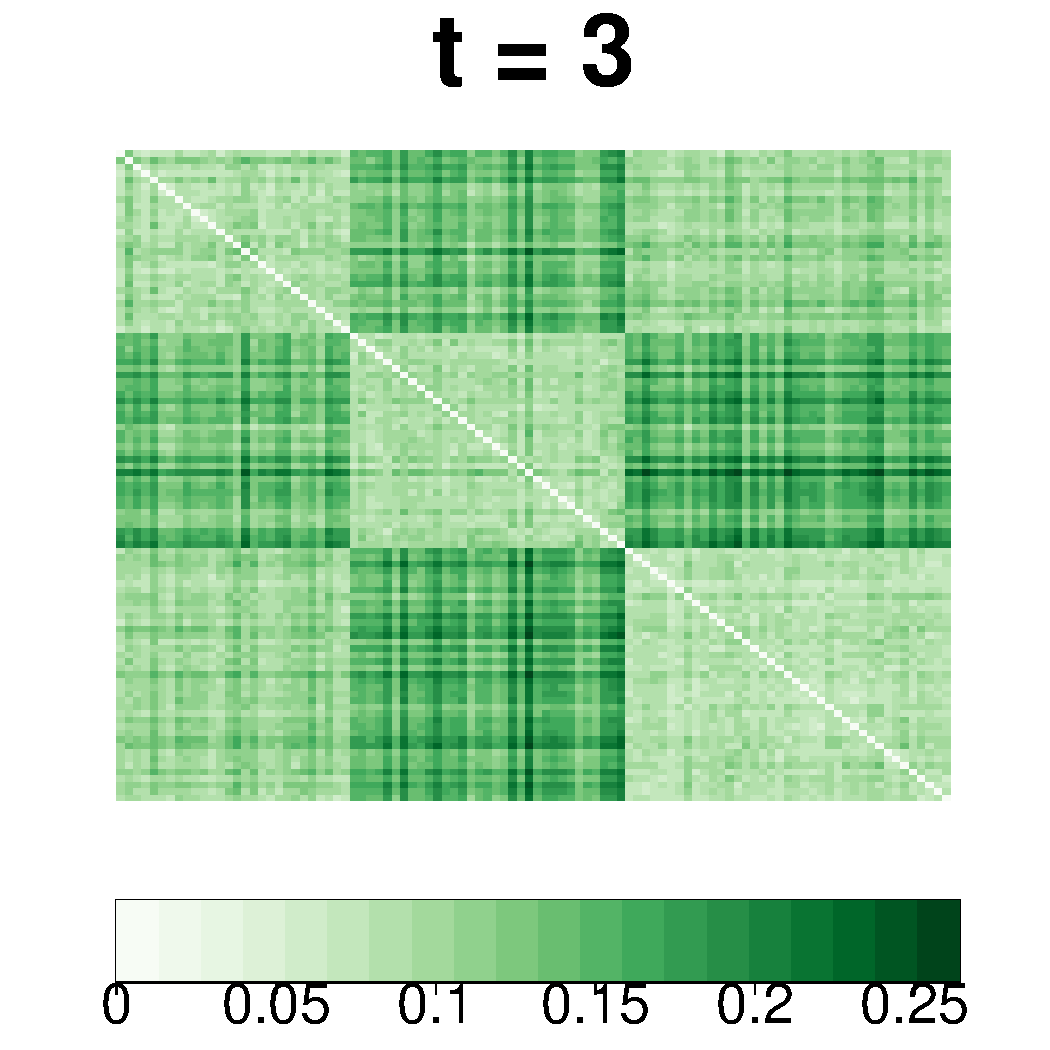
\includegraphics[width=0.3\linewidth]{../Figure/Dx3.pdf}
	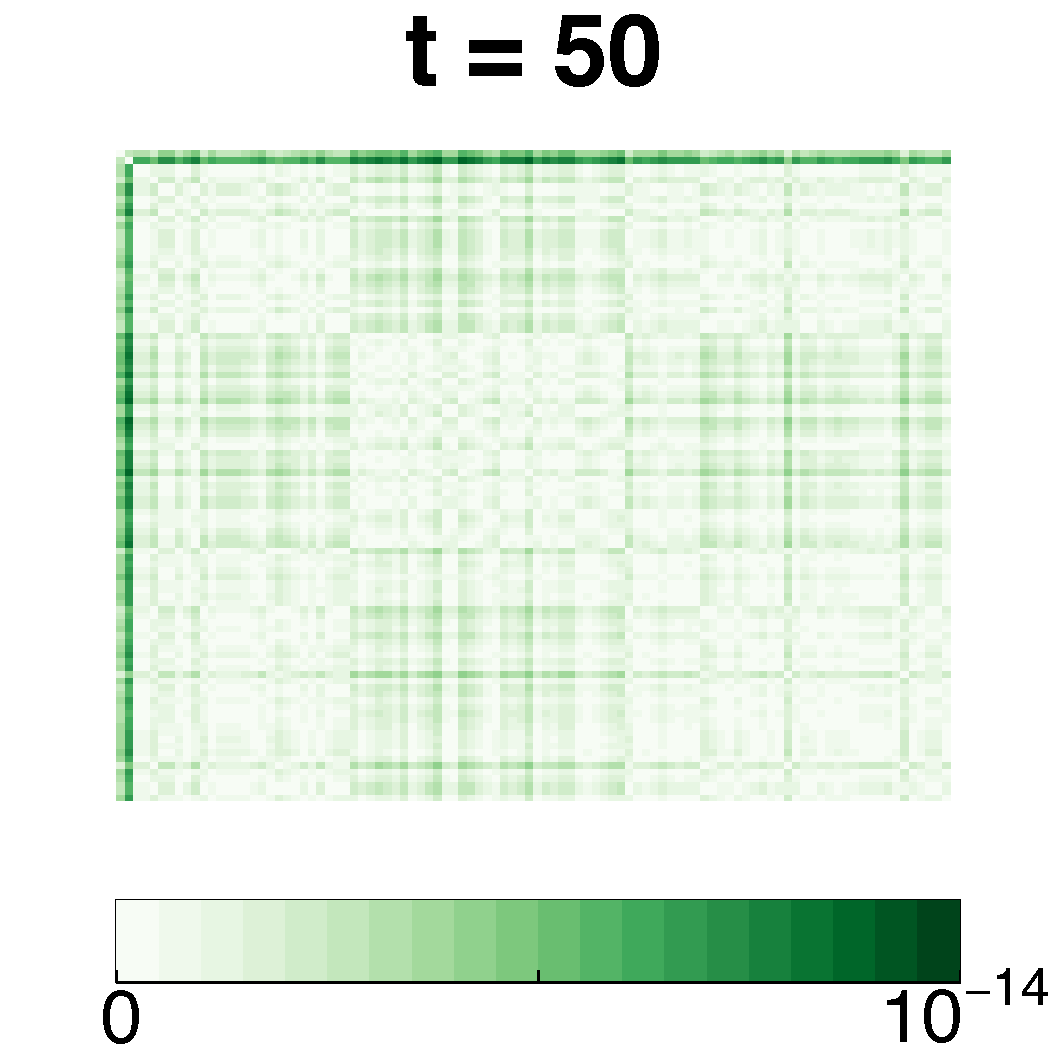
\includegraphics[width=0.3\linewidth]{../Figure/Dx50.pdf}
	\label{fig:diffusions}
	\caption{\textit{Diffusion matrix}, as a proposed alternative for Euclidean distance of $A$, provides \textbf{one-parameter family of network-based distances} where at early stage, e.g. at $t=1$, distance matrix is very similar to Euclidean distance of $A$ but as time goes by the pattern shown in the distance matrix changes, and \textbf{at optimal time point $t^{*} = 3$ distance matrix shows most clear block structures and at the same time it exhibits most dependence to distance matrix of $\mathbf{X}$.}}
\end{figure}	


\subsection*{Highest power of MGC under diffusion maps}

\begin{SCfigure}[][h]
	\centering
	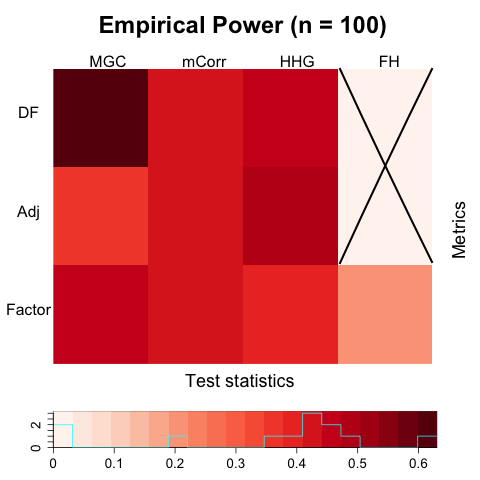
\includegraphics[width=0.38\paperwidth, height=0.33\paperwidth]{../Figure/ThreeSBM_results_simple.png}
	\caption{This power heatmap illustrates the superior power of multiscale generalized correlation (\texttt{MGC}) under diffusion distance matrix (\texttt{DF}) in three SBM (model~\ref{eq:Three}), compared to under adjacency matrix distance (\texttt{Adj}) or latent factor distance (\texttt{Factor}). \textbf{This demonstrates that especially in the presence of nonlinear network dependency, \texttt{MGC} statistic along with a family of diffusion distances catches non monotonic correlations efficiently than the other statistics and metrics.}}
	\label{fig:threeSBM}
\end{SCfigure}


\subsection*{Superiority of the proposed method under non-linear dependency}

\begin{figure}[h]
	\centering
	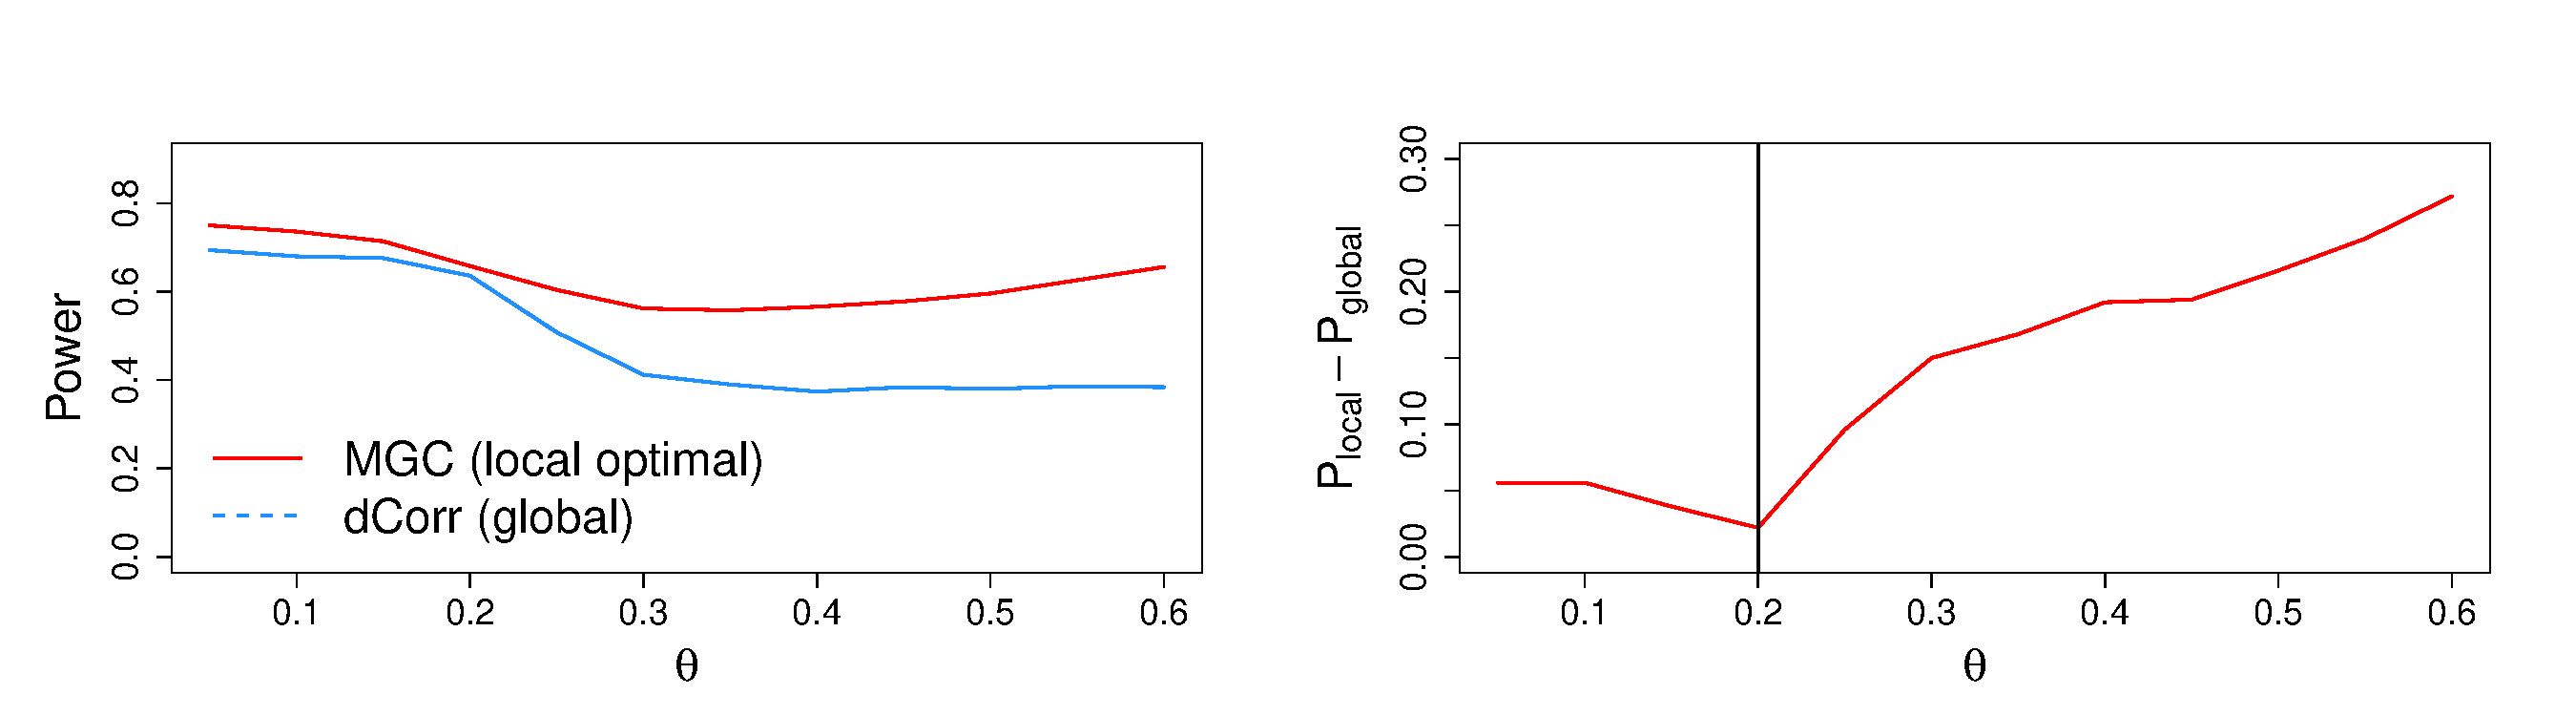
\includegraphics[width=\linewidth]{../Figure/powerplot_simple.pdf}
	\caption{X-axis of $\theta$ controls the existence/amount of nonlinear dependency and in this particular case nonlinearity exists when $\theta > 0.2$ and gets larger as it increases. You can see the discrepancy in power between global and local scale tests also gets larger accordingly, \textbf{mostly due to decreasing power of global test but relatively stable power of \texttt{MGC} under nonlinear dependency} as presented in the left panel.}
	\label{fig:powerplot}
\end{figure}


\subsection*{Degree-corrected SBM with increased variability in node distribution}	
\subsection*{Validity of the method even under competitor's model}

\begin{figure}[H]
	\centering
	\begin{subfigure}[b]{0.35\textwidth}
		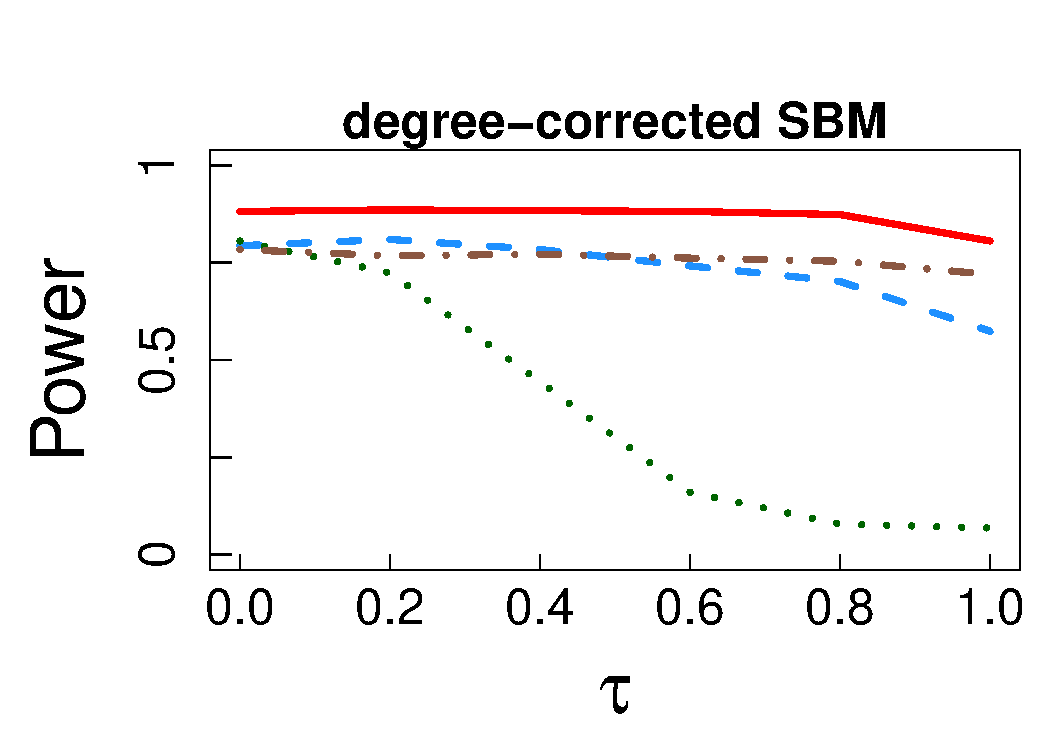
\includegraphics[width=\textwidth]{../Figure/onlytau.pdf}
		\caption{}
		\label{fig:dcSBM}
	\end{subfigure}
	\begin{subfigure}[b]{0.6\textwidth}
		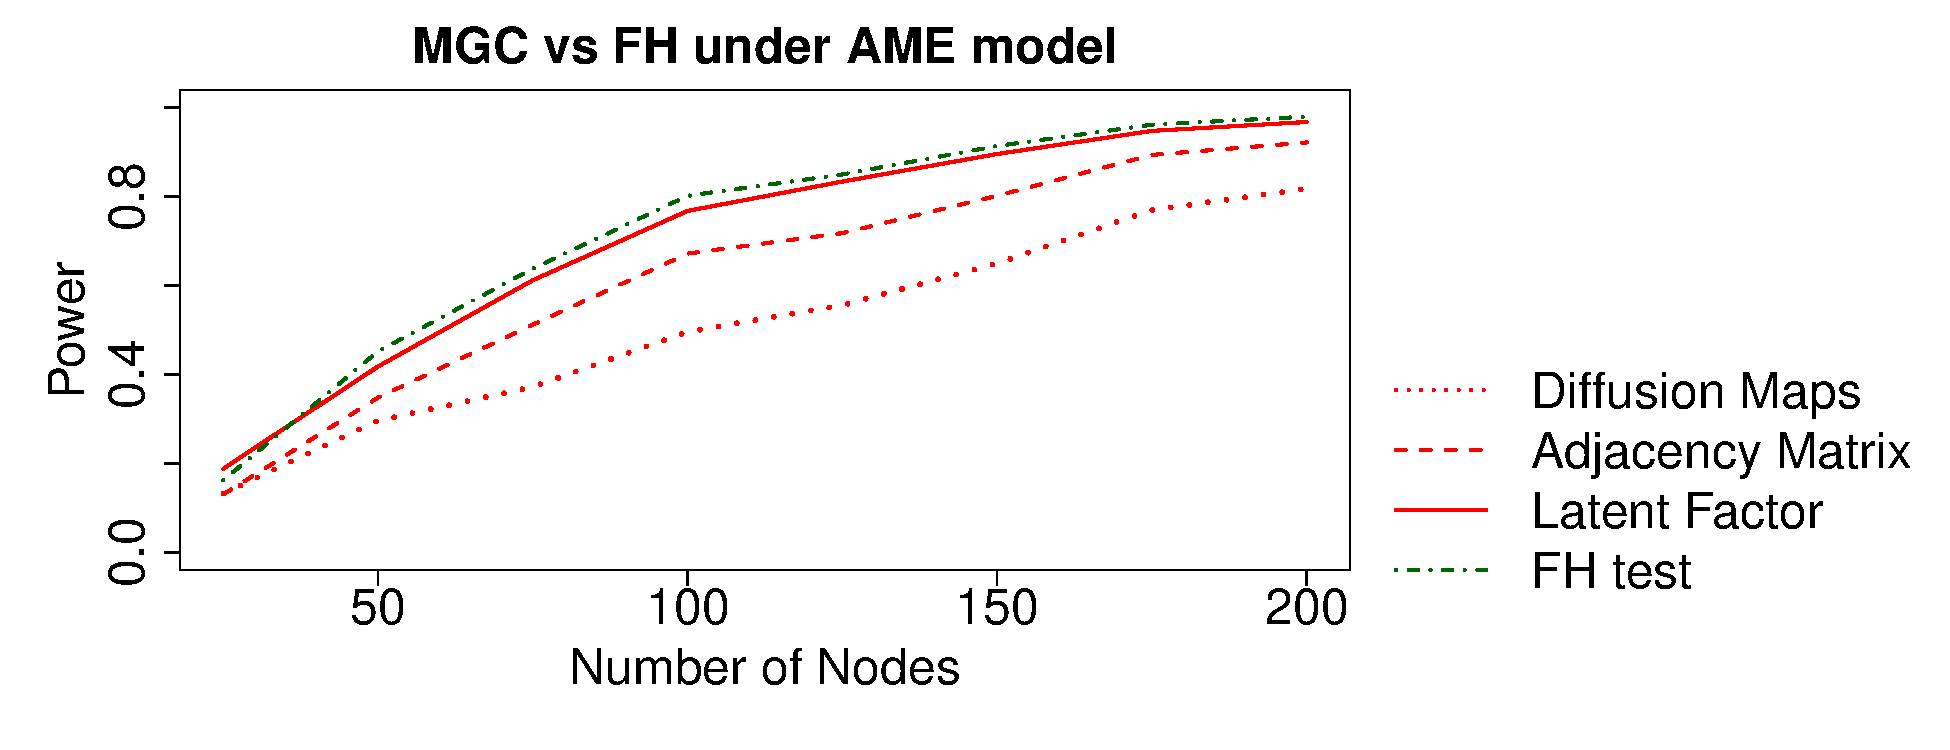
\includegraphics[width=\textwidth]{../Figure/ame_part.pdf}
		\caption{}
		\label{fig:ame}
	\end{subfigure}
	\caption{(a) In degree-corrected SBM where the variability in degree distribution increases as $\tau$ increases, testing power of diffusion maps are more likely to be robust against increasing variability compared to other network metrics, e.g. adjacency matrix or latent positions. \texttt{FH} test statistics allowing different dimensions of network factors perform consistently well but still have less power than \texttt{MGC}. (b) \texttt{MGC} utilizing diffusion distances loses some power under additive and multiplicative model which favors estimated latent position metrics, but \texttt{MGC} does as good as \texttt{FH} tests under latent factor metrics which closes to the truth. This reveals the flexibility in distance-based matrix in \texttt{MGC} statistics, which can be chosen depending on model fit or preliminary knowledge.}
	\label{fig:combined}
\end{figure}	


\subsection*{Node Contribution}

\begin{figure}[h]
	\centering
		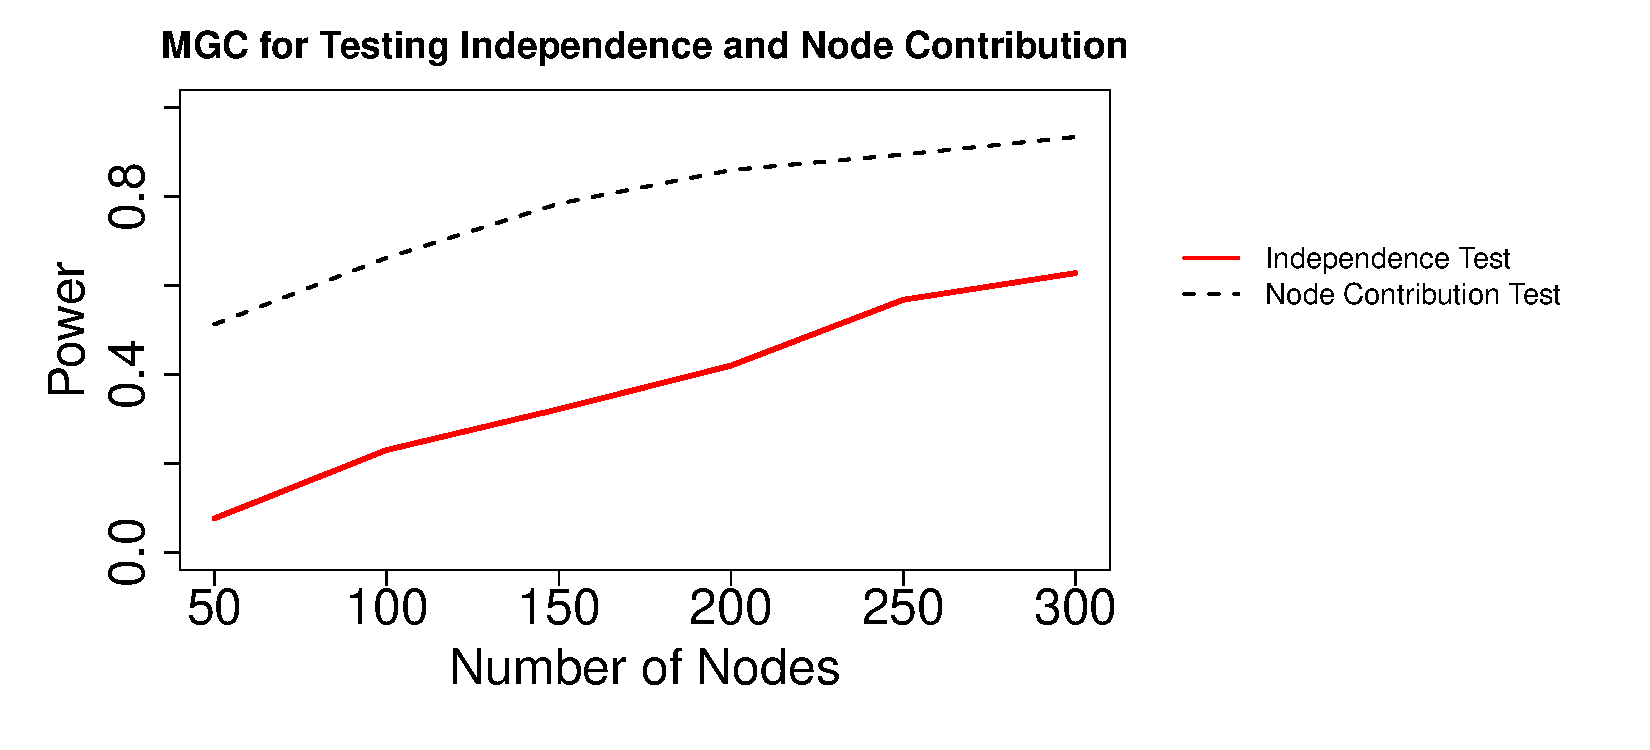
\includegraphics[width=0.8\linewidth]{../Figure/nodecontri.pdf}
	\caption{This plot describes both power of \texttt{MGC} and the rate of correctly-ranked node contribution increase as the number of nodes increases when only half of the nodes for each simulation actually are set to contribute to the independence test, \textbf{which validates the use of node contribution measure in independence test.}}
	\label{fig:contribution}
\end{figure}


\subsection*{Political Network}

\begin{figure}[H]
	\centering
		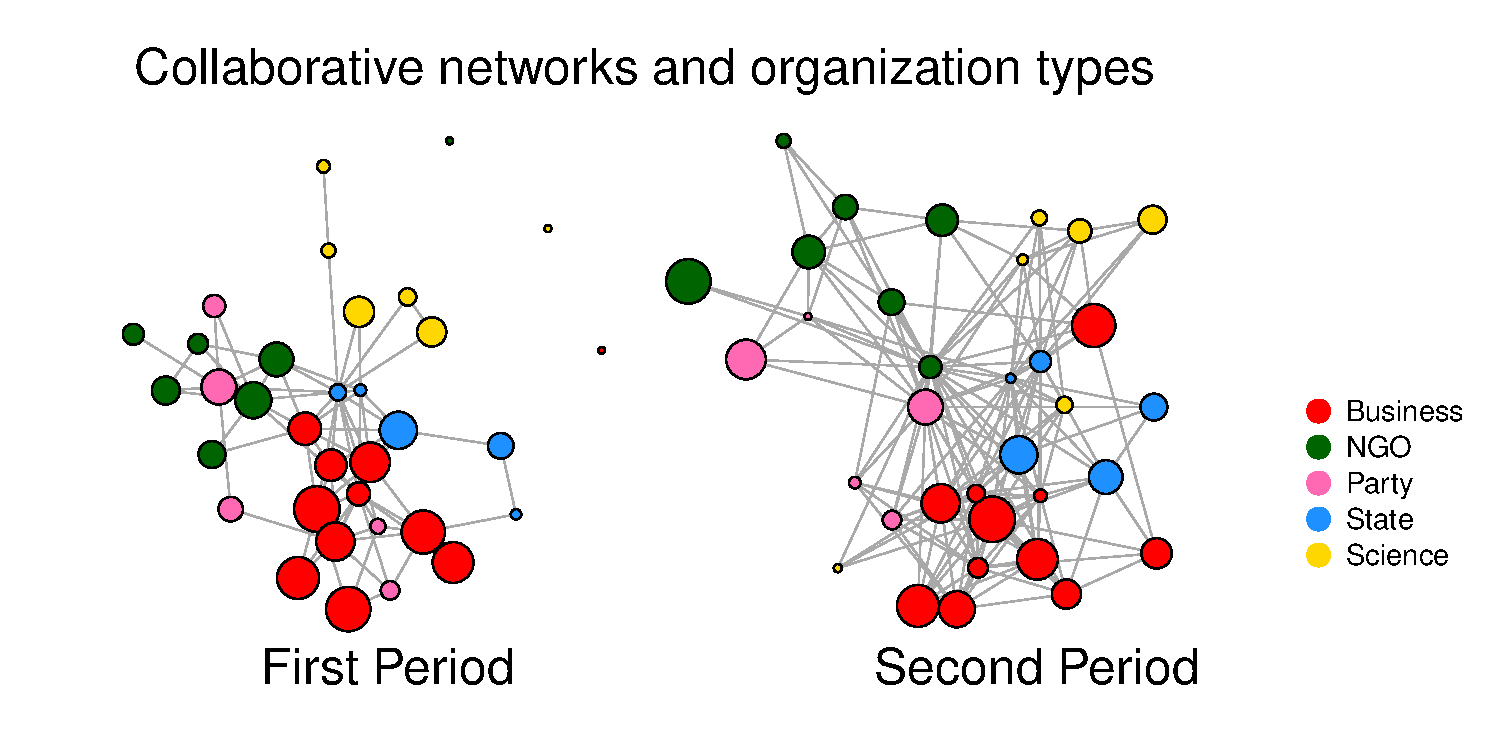
\includegraphics[width=\linewidth]{../Figure/two_politics.pdf}
	\caption{Both networks depict the collaboration network during the two time periods where it turns out significant network dependency in types of organizations. \textbf{Considering the size of nodes is proportional to the contribution to the statistic, you can notice that throughout all periods business sector is most actively collaborating within their group.}}
	\label{fig:politics}
\end{figure}

%%%%%%%%%%%%%%%%%%%%%%%%%%%%%%%%%%%%%%%%%%%%
\newpage
\section{Checklist}

\begin{itemize}

\item \textbf{1.  1 sentence summary}

We propose the nonparametric method to test independence between network and nodal attributes using multiscaled generalizing correlation with family of network-based distances applied.

$\rightarrow$ \textbf{title} : Testing independence in networks via family of network metrics


\item \textbf{2.  1 paragraph summary} 
\subitem \textbf{(i) big opportunity sentence}: Network data are ubiqutous.

\subitem \textbf{(ii) specific opportunity} : We are interested in investigating relationship between network topology and a random variable associated with each node.

\subitem \textbf{(iii) challenge sentence} : Network topology is high-dimensional data and there is often no standardized structure on network.

\subitem \textbf{(iv) gap sentence} : Network model-based approach fails to deal with increasing information having no standard pattern of network.

\subitem \textbf{(v)  action sentence} : Multiscale generalized correlation (MGC) statistic successfully detects the nature dependence between two data sets and we are going to utilize a family of network-based distances when implementing MGC in testing independence.

\subitem \textbf{(vi) resolution sentence} : As a result we have multiscale test statistics which provide the evidence of dependence between network and nodal attributes, more robust to nonlinear dependence and increased variability compared to the other statistics and other metrics.


\item \textbf{5 paragraph intro}

\subitem \textbf{(i) bulleted list of ~3-5 main factors that created an opportunity for your work.}

\subsubitem - Statisticians have long considered the problem of revealing the relationship between two different data sets.
\subsubitem - Among the data having diverse types and dimensions, network is now an ubiquitous dataset which is very likely to possess the properties of both high dimensionality and nonlinearity.
\subsubitem - Beyond the interest in network topology, we consider the relationship between network topology and a random variable associated with each node. 

\subitem \textbf{(ii) one sentence summary of the gap, that is, the key ingredient that is missing.}

 Network model-based statistics presumed that all nodes would exhibit the same pattern of dependence on their network relationship as specified in the model, which cannot be assured in network data.

\subitem \textbf{(iii) bulleted list of ~3-5 main challenges that must be overcome.}

\subsubitem -  Whatever the true nature of network is and however network is correlated with its nodal attributes, our testing statistics should aim at detecting significant association between network and nodal attributes.

\subsubitem - We have to consider increasing amount of information inherent in network data as the number of nodes increases. 

\subsubitem -  There exists an dependency among columns of an adjacency matrix so theoretically we cannot directly use an Euclidean distance of an adjacency matrix.


\subitem \textbf{2-3 sentence summary of what you did} 

First of all, considering the properties of network data, we propose applying multiscale generalized correlation statistics into testing network independence which deal with correlation between high-dimensional data sets which might have nonlinear dependence. However we confront with the difficulty in finding the valid iid node-specific coordinates of which Euclidean distance will be an ingredient for MGC statistics. We claim that diffusion maps derived from random walk on graph furnish robust network metrics against to increased variability in edge distributions as well as they satisfy theoretical constraints for a jointly exchangeable graph.


\subitem \textbf{2-3 sentence summary on how your work changes the world.}

Beyond the traditional setting of the data in independence test, i.e. two random vectors, we suggest the method to investigate unique but also ubiqutous data of network and its nodal attributes by utilizing the method testing two random vectors. By suggesting using a family of network metrics which are equipped with favored theoretical and practical properties, we are able to better understand relative locations of each node over network and also how the amount of dependency changes along with diffusion time. Moveover now away from the assumption on globally existing monotonic dependence, MGC with diffusion distances performs better than the other statistics or metrics under nonlinear dependence and we measure each node's contribution to detecting the dependence.

\item  \textbf{Outline of the results : list the evidence that supports that you filled the gap}

 Through simulation studies, we demonstrate that superiority of \texttt{MGC} statistics becomes more evident when the relationship between network and nodal attributes is not linear. Moreover diffusion distance matrix maintains its stability under increased variability in network better than an adjacent matrix or latent network factors from model-based methods. 


\item  \textbf{outline of discussion, to include:}
\subitem \textbf{(i) bulleted list of previous related work}

-  We proposed the method to test independence in network data without model assumption nor estimations. 

- Our methods work better than the others especially under nonlinear dependency, and we are able to measure each node's contribution to detecting dependence.

\subitem \textbf{(ii) bulleted list of potential extensions} 

- Since we did not suggest the method to derive the optimal diffusion time point but rather choose the one which shows highest power from $t=1$ to $t=10$, we can further study the algorithm that chooses the optimal diffusion time or diffusion matrix. 

- Both \texttt{MGC} and a family of diffusion distances are specialized in preserving local relationship between two data set. Based on this strength, we may preserve the true relationship between network and nodal attributes through investigating multiscale test statistics.

- We may utilize the diffusion maps from two networks and use them to test independence of network topology of two different networks with same nodes. 
  

\end{itemize}


\end{document}